\textbf{Experiments.} We swept the buffer size $N \in \{8, 64, 1024\}$ and the number of producers $P \in \{1, 2, 4, 8, 12, 15, 23, 31\}$,
keeping the total number of values fixed at $nP = 4$M ($n = 4\text{M}/P$), so that every point does the same amount of work and the times can be compared directly.
With the consumer there are $P+1$ threads, so $P \le 15$ fits in the 16 hardware threads, while $P = 23, 31$ oversubscribe the machine.
We ran those two points only once, with a 120\,s limit, because some busy-waiting runs became very slow there; all other points are the median of 3 runs.
In a second sweep we fixed $N=64$, $P=8$ and varied $n$ from 125k to 1M (1M to 8M values in total).

\begin{figure}[h]
\centering
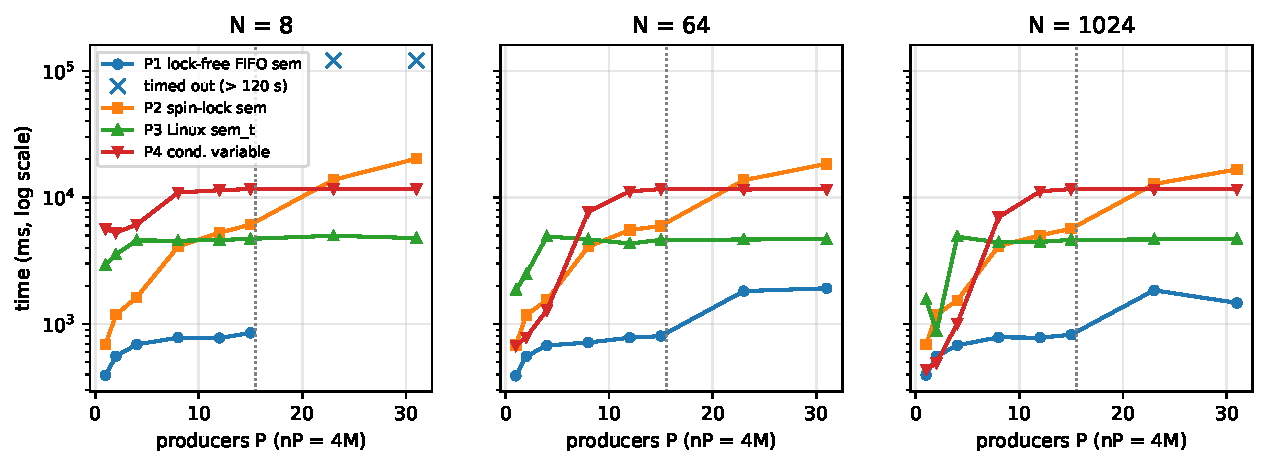
\includegraphics[width=\textwidth]{figs/q1_sweep.pdf}
\caption{Q1: time to pass 4M values from $P$ producers to one consumer (log scale; lower is better). The dotted line marks $P+1 = 16$ threads, the number of hardware threads.
An $\times$ means the run did not finish within 120\,s.}
\label{fig:q1}
\end{figure}

\begin{table}[h]
\centering\small
\begin{tabular}{rlrrrrrrrr}
\toprule
$N$ & Version & $P{=}1$ & $P{=}2$ & $P{=}4$ & $P{=}8$ & $P{=}12$ & $P{=}15$ & $P{=}23$ & $P{=}31$ \\
\midrule
8 & P1 & \textbf{393} & \textbf{557} & \textbf{690} & \textbf{781} & \textbf{775} & \textbf{852} & $>$120k & $>$120k \\
 & P2 & 687 & 1184 & 1623 & 4086 & 5261 & 6106 & 13778 & 20222 \\
 & P3 & 2908 & 3542 & 4577 & 4550 & 4609 & 4709 & \textbf{4982} & \textbf{4769} \\
 & P4 & 5617 & 5272 & 6102 & 10921 & 11409 & 11649 & 11739 & 11671 \\
\midrule
64 & P1 & \textbf{390} & \textbf{556} & \textbf{676} & \textbf{715} & \textbf{779} & \textbf{803} & \textbf{1819} & \textbf{1916} \\
 & P2 & 682 & 1177 & 1548 & 4091 & 5520 & 5966 & 13684 & 18420 \\
 & P3 & 1854 & 2476 & 4915 & 4667 & 4321 & 4619 & 4652 & 4677 \\
 & P4 & 675 & 785 & 1288 & 7713 & 11164 & 11644 & 11561 & 11598 \\
\midrule
1024 & P1 & \textbf{395} & 556 & \textbf{679} & \textbf{785} & \textbf{780} & \textbf{823} & \textbf{1849} & \textbf{1467} \\
 & P2 & 692 & 1184 & 1540 & 4125 & 5020 & 5662 & 12767 & 16658 \\
 & P3 & 1566 & 876 & 4893 & 4412 & 4449 & 4622 & 4659 & 4688 \\
 & P4 & 437 & \textbf{492} & 1005 & 6986 & 11186 & 11646 & 11566 & 11607 \\
\bottomrule
\end{tabular}

\caption{Q1: time in ms for $nP = 4$M values (median of 3; single run for $P \ge 23$). Bold marks the fastest version for each $(N, P)$.}
\label{tab:q1}
\end{table}

\paragraph{P1 with up to 15 producers.}
For every $N$ and every $P \le 15$, P1 was the fastest of the four versions, except at $P = 2$ with $N = 1024$ (discussed under P4 below).
Its time went from 0.39\,s at $P=1$ to 0.80--0.85\,s at $P=15$, i.e.\ about 100--215\,ns per value. At $P=15$ it was 7--7.5$\times$ faster than P2,
5.5--5.8$\times$ faster than P3 and 14--14.5$\times$ faster than P4. We think this comes mainly from three properties of the design:
in the common case \texttt{wait} and \texttt{post} are a single successful CAS each, with no lock to hand over between threads;
waiting threads only read \texttt{grant}, and each \texttt{post} lets exactly one waiter through, so waiters do not compete with each other;
and no thread ever enters the kernel.

\paragraph{P2.}
P2's time grew almost linearly with $P$, from 0.68--0.69\,s at $P=1$ to 5.7--6.1\,s at $P=15$. Our understanding is that all producers that see a positive count
compete for the same lock, and the consumer's \texttt{post} has to win that lock against them before any producer can continue. The test-and-test-and-set lock with
back-off reduced this (Section~1.2) but did not remove it. P2 also slowed down a lot when oversubscribed (13--20\,s at $P = 23, 31$),
which we attribute to lock holders being preempted while the other threads spin.

\paragraph{P3.}
From $P = 4$ on, P3 took 4.3--5.0\,s regardless of $P$ or $N$. We believe that with several producers the semaphore is almost always contended,
so most \texttt{sem\_wait} calls sleep and most \texttt{sem\_post} calls have to wake a sleeper through a system call, which costs on the order of a microsecond per value.
Because sleeping threads do not use the CPU, its time did not change between $P = 15$ and $P = 31$. With a single producer, $N$ made a difference
(2.9\,s at $N=8$ vs 1.6\,s at $N=1024$), presumably because a small buffer fills up immediately and forces the producer to sleep more often.

\paragraph{P4.}
P4 was the slowest version for $P \ge 8$, levelling off at about 11.6\,s. Every \texttt{wait} and \texttt{post} takes the semaphore's mutex, so at this point
up to 15 producers and the consumer queue on one mutex, and a woken waiter has to take the mutex again before it can continue.
With two producers and $N = 1024$, however, P4 was the fastest version (0.49\,s vs 0.56\,s for P1), and with one producer it came close (0.44\,s vs 0.40\,s). In that setting threads rarely have to wait in either version.
One possible explanation, which we have not verified, is that P1's \texttt{FetchAndInc} loads the counter and then does the CAS, which may cost an extra cache-line transfer
when another core wrote the line last, whereas glibc's mutex fast path is a single CAS.

\paragraph{P1 with more threads than hardware threads.}
The result we found most surprising was P1 at $N = 8$ with $P = 23$ and $P = 31$: it did not finish within 120\,s (in an earlier trial a single
$P=23$ run took about 560\,s), while P3 needed under 5\,s. Our explanation is that this follows from combining strict FIFO order with busy-waiting.
With 24 or more threads on 16 hardware threads, some threads are always preempted. A \texttt{post} lets through only the thread holding the next ticket;
if that thread is not running, nobody can use the free slot until the scheduler runs it again, while the other waiters, who may not overtake it, keep spinning.
With $N = 8$ almost all producers are waiting on \texttt{sem\_prod} at any time, so this would happen on almost every value.
With $N = 64$ or $1024$, P1 still finished (1.5--1.9\,s), although more slowly than at $P = 15$. P3 sleeps instead of spinning and was not affected.
We also checked this on fewer CPUs (restricting the program with \texttt{taskset}). With 4 CPUs, P1 was fine with up to 8 producers (0.1--0.3\,s for 1M values),
but with $N = 8$ and $P = 15$ it did not finish 1M values within 60\,s.

As an experiment, we tried a variant of P1 that calls \texttt{sched\_yield()} when a waiter (or the consumer, waiting on a \texttt{full} flag) has spun for a while without progress,
so that a preempted thread can run sooner. FIFO order is unchanged, since the tickets are the same. This removed the problem in our tests (4M values, median of 3: 8.1\,s with 4 CPUs, $N=8$, $P=15$;
3.7\,s and 6.0\,s with 16 CPUs, $N=8$, $P=23$ and $31$) and did not slow down the normal cases (it was even slightly faster: 0.67--0.70\,s vs 0.78--0.80\,s at $N=64$, $P=8, 15$).
However, \texttt{sched\_yield()} gives the CPU to another thread, and the assignment asks that the waiting thread is not context-switched,
so we did not include it in the submitted P1. This means our P1 is best run with $P+1$ at most the number of hardware threads, or with a larger $N$;
with far more threads than cores and a small buffer, it can take minutes.

\paragraph{Effect of $n$.}
\begin{figure}[h]
\centering
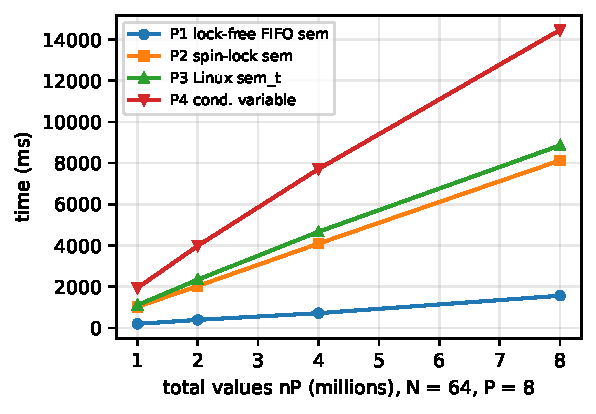
\includegraphics[width=0.45\textwidth]{figs/q1_n.pdf}
\caption{Q1: time vs total number of values ($N = 64$, $P = 8$).}
\label{fig:q1n}
\end{figure}
For every version, the time grew linearly with the number of values (Figure~\ref{fig:q1n}; P1: 0.20, 0.39, 0.72, 1.56\,s for 1, 2, 4, 8M values).
So the cost per value is roughly constant, and we think the 4M values used in the main sweep (at least 0.5\,s per run) are enough to average out measurement noise.
The ranking of the four versions did not depend on $n$.

\paragraph{Testing the FIFO guarantee.}
To check the FIFO property directly, we wrote a separate test program (not included in the submission) that reuses the four semaphores from \texttt{q1\_mpsc.cpp} unchanged.
The semaphore starts at 1, so only one thread passes at a time. $T$ threads each repeat
\emph{take an arrival number (\texttt{FetchAndInc}), \texttt{wait}, log the arrival number, short critical section, \texttt{post}},
for $160{,}000$ passes in total. We count the passes that were \emph{overtaken} (some later arrival passed first), and the worst \emph{bypass}
(the largest number of later arrivals that passed before one thread).

\begin{center}\small
\begin{tabular}{rcccc}
\toprule
$T$ & P1 lock-free FIFO & P2 spin lock & P3 \texttt{sem\_t} & P4 cond.\ var. \\
\midrule
4  & 2 \;(0.001\%), max 2  & 38.4\%, max 81   & 49.7\%, max 941 & 34.6\%, max 779 \\
8  & 1 \;(0.001\%), max 2  & 43.7\%, max 377  & 55.3\%, max 747 & 43.7\%, max 722 \\
15 & 1 \;(0.001\%), max 51 & 60.4\%, max 2491 & 58.3\%, max 848 & 44.8\%, max 424 \\
\bottomrule
\end{tabular}

\smallskip
{\footnotesize Overtaken passes (median of 3 runs) and worst bypass over the 3 runs.}
\end{center}

For P1, at most 5 of the 160{,}000 passes were overtaken in any run. We think these few cases come from the test itself rather than the semaphore:
the arrival number is taken just \emph{before} \texttt{wait} takes its ticket, so a thread that is delayed between the two (for example, by an interrupt) can be overtaken.
This would also explain the single bypass of 51 in one run at $T=15$. The other three semaphores do not promise any order, and in our runs
34--61\% of their passes were overtaken, with single waiters bypassed by hundreds or, in one case, thousands of later arrivals.

\paragraph{Fairness in the producer-consumer program.}
We also wanted to see whether FIFO order makes the producers progress at the same rate. In the real program ($N=64$, $nP=4$M) we recorded when each producer finished,
and report the first producer's finish time as a fraction of the total time (1.0 means all producers finished together; median of 3 runs):

\begin{center}\small
\begin{tabular}{rcccc}
\toprule
$P$ & P1 & P2 & P3 & P4 \\
\midrule
4  & 0.978 & 0.954 & 0.990 & 0.989 \\
8  & 0.999 & 0.879 & 0.970 & 0.995 \\
15 & 0.993 & 0.820 & 0.994 & 0.990 \\
\bottomrule
\end{tabular}
\end{center}

P2 was noticeably unfair, increasingly so with more producers: some producers finished well before others, and in the worst run the first producer was done after only 80\% of the total time.
P1 kept all producers within a few percent of each other. We expected P3 and P4 to be less fair than P1, but over a whole run they were about as fair, even though their individual passes are often out of order.
Our guess is that their reorderings average out over millions of passes, while P2's lock tends to favour the same threads (for example, the thread that has just released the lock may win it again).
So in our measurements, the benefit of FIFO showed up mostly in the waiting time of individual \texttt{wait} calls, and P2 was the only version that was also unfair over a whole run.

\paragraph{Effect of padding the shared variables.}
Late in the project we noticed that \texttt{write\_pointer} and the two semaphores were ordinary neighbouring global variables, so they shared a cache line with each other
and with \texttt{N}, \texttt{n} and \texttt{array}, which every thread reads for every value. We gave each of them its own cache line (Section~1.3) and reran all the experiments
above; all other numbers in this section are from the padded version. To measure the effect itself, we ran the unpadded and the padded build alternately in one session
($N = 8, 64, 1024$; $P = 1, 2$, plus $P = 4, 8, 15$ for $N = 8, 64$; median of 3 each).
P1 became 27--28\% faster at $P=1$ (0.54\,s $\to$ 0.39\,s) and 18--20\% faster at $P=2$ (0.69--0.70\,s $\to$ 0.56\,s), for every $N$.
Our guess is that before, every \texttt{FetchAndInc(\&write\_pointer)} by a producer invalidated the line holding \texttt{N}, which the consumer then had to fetch again.
P2 became 5--29\% faster for $P \ge 2$, which we think is because the two semaphores' locks no longer share a line, so producers spinning on \texttt{sem\_prod}
no longer slow down the consumer's \texttt{sem\_cons}. P3 changed in both directions: with one producer it became 20\% slower at $N = 64$ and $1024$
(1.55\,s $\to$ 1.86\,s and 1.21\,s $\to$ 1.45\,s), but with two producers at $N=64$ it became 33\% faster (2.96\,s $\to$ 1.99\,s). P4 with two producers at $N=1024$
became 17\% slower (0.42\,s $\to$ 0.49\,s). With so few threads every value goes through both semaphores, so perhaps keeping them on one line sometimes meant fewer
cache-line transfers; we do not have a clear explanation for these P3 and P4 cases. All other points we compared changed by less than 10\%, and apart from P1 now also being
fastest at $P=1$, $N=1024$, the ranking of the four versions did not change.
